% Read the readme first!
% options:
% - uulm-draft: show todonotes, links, linenumbers hide label names
% - uulm-draft-verbose: show todonotes, links, linenumbers, label names
% - uulm-release-electronic: show links, hide todonotes, linenumbers, label names
% - uulm-release-print hide everything
%

\documentclass[uulm-release-electronic]{thesis-uulm} % für die finale Abgabe
%\documentclass[uulm-draft]{thesis-uulm} % um ToDo's anzuzeigen

% workarround for some stupid error in combination with IEEEtran, bibtex and babel.
\makeatletter
\def\markboth#1#2{%
  \def\leftmark{\@IEEEcompsoconly{\sffamily}#1}%
  \def\rightmark{\@IEEEcompsoconly{\sffamily}#2}}
\makeatother

% Choose language
\usepackage[ngerman]{babel}
%% \usepackage[english]{babel}

% Fonts
\renewcommand{\sfdefault}{phv}
\renewcommand{\rmdefault}{phv}
\renewcommand{\ttdefault}{pcr}

% Adjust variables
\author{Vorname Nachname}
\title{Titel der Arbeit}
\email{vorname.nachname@uni-ulm.de}
\matnr{1234567}	% Student ID

\type{Seminararbeit} % Type of Thesis (Bachelors, Masters)
\jahr{Wintersemester 2017/18}

\gutachterA{Prof. Dr. Timo Ropinski} % First Reviewer
%\gutachterB{Prof. Dr. Un Leserlich}  % Second reviewer
\betreuer{Julian Kreiser} % supervisor

% Can be user to only compile parts of the document
\includeonly{
template/definitions,
chapters/introduction,
chapters/related-work,
chapters/content,
chapters/evaluation,
chapters/conclusion,
chapters/appendix
}

% Definitions for code listings
%% definitions.tex
%%

%Listings für die Darstellung der Treiber im Anhang:
%-------------------------------------------------------
\usepackage{listings}

\usepackage{color}
\definecolor{gray}{rgb}{0.4,0.4,0.4}
\definecolor{darkblue}{rgb}{0.0,0.0,0.6}
\definecolor{cyan}{rgb}{0.0,0.6,0.6}

\lstset{
  basicstyle=\ttfamily,
  columns=fullflexible,
  showstringspaces=false,
  commentstyle=\color{gray}\upshape
}

\lstdefinelanguage{XML}
{
  morestring=[b]",
  morestring=[s]{>}{<},
  morecomment=[s]{<?}{?>},
  stringstyle=\color{black},
  identifierstyle=\color{darkblue},
  keywordstyle=\color{cyan},
  morekeywords={xmlns,version,type}% list your attributes here
}
%-----------------------------------------------------------


\begin{document}

\frontmatter %%%%%%%%%%%%%%%%%%%%%%%%%%%%%%%%%%%%%%%%%%%%%%%%%%%%%%%%%%%%%%%%%
\pagenumbering{roman}
\begin{nolinenumbers}
\maketitle

\copyrightpage % comment out if not wanted
\end{nolinenumbers}

\setstretch{1.2}

\begin{nolinenumbers}
\tableofcontents
\end{nolinenumbers}

\mainmatter %%%%%%%%%%%%%%%%%%%%%%%%%%%%%%%%%%%%%%%%%%%%%%%%%%%%%%%%%%%%%%%%%%
\pagenumbering{arabic}
%% introduction.tex
%%

\chapter{Einleitung}
\label{ch:introduction}

Seit jeher werden Landkarten genutzt, um die topologische Beschaffenheit der Welt sowie, vor allem in Zeiten der Globalisierung, (über-)regionale Sachverhalte und Statistiken grafisch aufbereitet darzustellen.

Allerdings bestehen zwei Problematiken. Dreidimensionale Strukturen wie Globen (und damit auch deren Oberflächen) können aufgrund des "Verlusts" einer Dimension grundsätzlich nur verzerrt auf zweidimensionalen Strukturen (wie Papier oder Computer-Bildschirmen) wiedergegeben werden. Außerdem gibt es unzählige Möglichkeiten, eine solche Verzerrung durchzuführen. Die Vereinheitlichung einer solchen Verzerrung (in Form einer Funktion) nennt man Projektion.

Die vorliegende Ausarbeitung beschäftigt sich mit solchen Projektionen. Es werden zunächst Projektionen im Allgemeinen und danach deren Implementierung und Nutzung in der JavaScript-Bibliothek D3.js erläutert.


%% related-work.tex
%%

\chapter{Verwandte Arbeiten}
\label{ch:verwandte-arbeiten}

Mit dem Befehl
\begin{verbatim}
\cite{}
\end{verbatim}

lassen sich Verweise auf Einträge in der Datei $bibliography.bib$ setzen um damit Zitate zu erzeugen.

Diese Zitate werden dann folgendermaßen im Text dargestellt:~\cite{kopka} und ein Eintrag im Literaturverzeichnis angelegt.

Hierbei gilt es zu beachten, dass Zitate grammatikalisch unsichtbar sind und dahier kein Teil des Satzes darstellen.
Deshalb sind Sätze wie:
\\
\\
In~\cite{Knappen2009} wurde gezeigt, dass\ldots
\\
\\
in jedem Fall zu vermeiden!
Stattdessen wird dies wie folgt geschrieben:
\\
\\
Knappen konnte in seiner Arbeit zeigen, dass LaTex sehr gut für Abschlussarbeiten geeignet ist~\cite{Knappen2009}.

%% content.tex
%%
\chapter{Illustrationen}
\label{ch:illustrationen}

\section{Bilder}
\label{ch:illustrationen:sec:images}

Bilder kann man natürlich auch in Arbeiten integrieren.
Für Fotos und Ähnliches unterstützt PDF-\LaTeX{} direkt \verb|jpg| und \verb|png|, ansonsten empfiehlt es sich Vektorgrafiken zu verwenden und diese als \verb|pdf| zu speichern.
Sollte ein Bild einmal zu viel weißen Raum um sich haben, so kann man mit dem Werkzeug \verb|pdfcrop| das Bild automatisch ausschneiden\cite{pdfcrop}.

\begin{figure} [ht]
\centering
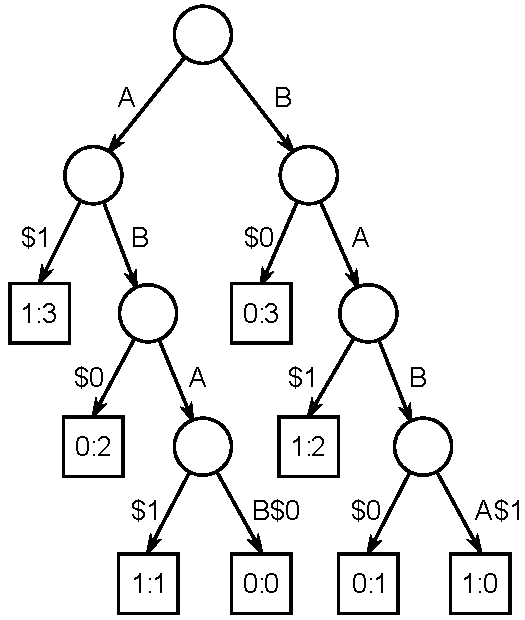
\includegraphics[width=.4\textwidth]{images/Suffix_tree_ABAB_BABA}
\caption{Beschreibung/Beschriftung des Bilds}
\label{fig:bild1}
\end{figure}

Mit Hilfe eines Labels kann man sich dann im Text auf diese Grafik (\ref{fig:bild1}) beziehen. 

\section{Tabellen}
\label{ch:illustrationen:sec:tables}

Seite \pageref{tab:beispieltabelle} enthält Beispieltabelle \ref{tab:beispieltabelle}.
In jedem \LaTeX{}-Buch finden sich gute Anleitungen zum Erstellen von Tabellen.
Komplexere Tabellen können in Excel vorgefertigt und mit Excel2LaTeX, einem Add-in von Excel, nach LaTeX konvertiert werden.

\begin{table}[h]
\begin{center}
\begin{tabular}{|l|l|l|}
	A & B & C \\\hline
	x & x & x \\
	x & x & x
\end{tabular}
\end{center}
\caption{Eine kleine Beispieltabelle}
\label{tab:beispieltabelle}
\end{table}

\section{Formeln}
\label{ch:illustrationen:sec:formula}

sec Formeln lassen sich in der Umgebung  \verb|math| erzeugen.
Die Kurz- Schreibweise lautet \verb|\( a^2+b^2=c^2 \)|;  hierbei steht die Formel dann im laufenden Text: \( a^2+b^2=c^2 \).
Die kürzeste Form ist mit zwei \verb|$| um die Formel, z.B.~so: Wasser ist H$_2$O.

Mit der Schreibweise \verb|\[ y=x^2 \]| wird die Formel mittig in einer eigenen Zeile gesetzt, z.B.

\[y = x^2 \]

Formeln in der Umgebung \verb|equation| werden mittig in einer eigenen Zeile gesetzt und fortlaufend nummeriert:

\begin{equation}
x_{1,2} = \frac{-b\pm\sqrt{b^2-4ac}}{2a}
\label{mitternachtsformel}
\end{equation}
Wenn wir z.B.~über die beliebte Mitternachtsformel (Gleichung \ref{mitternachtsformel}) Details im umliegenden Text schreiben wollen, lässt sich diese wie ein Bild referenzieren.

\section{Quellcode}
\label{ch:illustrationen:sec:code}

Quellcode und ähnlich zu formatierende Texte können mit \verb|verbatim| in einer Umgebung gesetzt werden.

\begin{verbatim}
Dieser Text ist in Schreibmaschinenschrift
\end{verbatim}

Schöner geht es mit dem \verb|listings|-Paket, das Quelltext auch entsprechend formatiert.
Dazu kann man in der Präambel die Sprache angeben, in der die Quellcodes geschrieben sind.

\begin{lstlisting}
public class Hello {
    public static void main(String[] args) {
        System.out.println("Hello World");
    }
}
\end{lstlisting}

Im Text gibt man Wörter am Besten als \verb|\verb##| an, dabei erwartet \LaTeX{} zweimal das gleiche Zeichen als Begrenzer.
Im Beispiel ist dies die Raute \verb|#|, man kann aber ein anderes Zeichen nehmen, z.B. das Plus .

\section{Text}
\label{ch:illustrationen:sec:text}

Text kann mit dem Befehl \verb|\emph{}| \emph{hervorgehoben} werden.
Falls in einem Satz ein Punkt vorkommt, macht man vor ihm kein Leerzeichen sondern eine Tilde (\verb|~|), denn dann fügt \LaTeX{} den korrekten Abstand ein, z.B.~so.

\begin{verbatim}
z.B.~so
\end{verbatim}

In der Präambel der vorliegenden tex-Datei gibt es den Befehl \verb|hypenation|, der zur Silbentrennung da ist.
\LaTeX{} verfügt zwar über  eine eingebaute Silbentrennung, die jedoch bei manchen Wörtern falsch trennt.
Damit diese Wörter korrekt getrennt werden, gibt man sie dann mit dem Befehl in der Präambel an\footnote{Das Wort \emph{Silbentrennung} ist hier das Beispiel}.

Fußnoten werden mit dem Befehl \verb|footnote| mitten in den fortlaufenden Text eingefügt. \footnote{Wie man schon im vorherigen Absatz sehen konnte.}.

In wissenschaftlichen Arbeiten muss man des öfteren andere Arbeiten zitieren.
Dazu nutzt man den Befehl \verb|\cite{name}|.
In eckigen Klammern kann man noch die Seitenzahl angeben, falls notwendig.
Der Name ist ein Schlüssel aus der Datei \verb|bibliography.bib| \cite[S.~10]{kopka}.
Falls einmal ein Werk nur indirekt zu einem Teil der Arbeit beigetragen hat, kann man es auch mit \verb|nocite| angeben, dann landet es in der Literaturliste, ohne dass es im Text ausdrücklich zitert wird.

\subsection{Weiterführendes}

Zum Schluss sei auf die Vielzahl an Büchern zu \LaTeX{} verwiesen.
In jeder Bibliothek wird sich eine Einführung finden, in der dann weitere Themen wie mathematische Formeln, Aufbau von Briefen und viele nützliche Erweiterungen besprochen werden.

%% evaluation.tex
%%

\chapter{Abschluss}
\label{ch:conclusion}

Wie in dieser Arbeit gezeigt wurde, kann in D3.js ohne großen Aufwand eine Landkarte erstellt und nach Belieben eingefärbt werden. Abschließend gilt zu sagen, dass die Möglichkeit besteht, Landkarten jeder Art in D3.js beliebig zu gestalten, und man keinesfalls auf rein optische Vorgänge beschränkt ist. 

So ist zum Beispiel eine interaktive Gestaltung der Karte innerhalb von D3.js möglich, indem man gezeichneten Pfaden Maus- oder sonstige Ereignisse und deren Verarbeitung zuweist. In entsprechender Fachliteratur wie der offiziellen Dokumentation finden sich viele weitere Ansätze zur Gestaltung.
%% conclusion.tex
%%

%% ==============================
\chapter{Fazit / Zusammenfassung}
\label{ch:conclusion}
%% ==============================

Lorem ipsum dolor sit amet, consetetur sadipscing elitr, sed diam nonumy eirmod tempor invidunt ut labore et dolore magna aliquyam erat, sed diam voluptua.
At vero eos et accusam et justo duo dolores et ea rebum.
Stet clita kasd gubergren, no sea takimata sanctus est Lorem ipsum dolor sit amet.
Lorem ipsum dolor sit amet, consetetur sadipscing elitr, sed diam nonumy eirmod tempor invidunt ut labore et dolore magna aliquyam erat, sed diam voluptua.
At vero eos et accusam et justo duo dolores et ea rebum.
Stet clita kasd gubergren, no sea takimata sanctus est Lorem ipsum dolor sit amet.
Lorem ipsum dolor sit amet, consetetur sadipscing elitr, sed diam nonumy eirmod tempor invidunt ut labore et dolore magna aliquyam erat, sed diam voluptua.
At vero eos et accusam et justo duo dolores et ea rebum.
Stet clita kasd gubergren, no sea takimata sanctus est Lorem ipsum dolor sit amet.


\backmatter %%%%%%%%%%%%%%%%%%%%%%%%%%%%%%%%%%%%%%%%%%%%%%%%%%%%%%%%%%%%%%%%%%

%\bibliographystyle{natdin}
\bibliographystyle{IEEEtranS}	% alternativer Stil
\bibliography{bibliography} % Bib-Datei

\end{document}
